%title page
\begin{frame}
\titlepage
\end{frame}

\begin{frame}{Introduction: The secret life of the astroparticle data}
%или "Астрофизика - современное состояние"))
\small
\begin{columns}
  \begin{column}[t]{0.45\textwidth}
    \begin{center}
      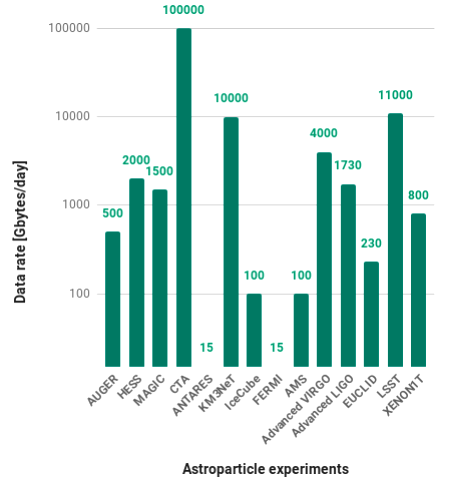
\includegraphics[width=0.79\linewidth]{pics/appec_base4.png}
    \end{center}
    \vspace{-2\parsep}
    \small Modern astroparticle experiments data rate [Gbytes/day]\footnotemark[1] %, source: APPEC brochure on Computing, 2016}
  \end{column}
  \hfill
  \begin{column}[t]{0.53\textwidth}
    % \vspace{1.5em}
    % Вступление - такие вступление :)
    % Современная астрофизика представлена большим количеством экспериментов, которые изучают примерно одно и то же (а зачастую - и прям совсем одно и то же, в плане объекта), но по-разному - т.е., в разных природных условиях и с использованием разных типов детекторов.
    % Каждый год данных прибывает, и при этом общй дата пул ежегодно растет, как на дрожжах (см. картинку)
    \begin{itemize}
    \item Wide range of experiments;
    \item Looking at the same sky with diffrent eyes: different detectors, different reactions under the study;
    \item Common data rate for astrophysical experiments all together is a few PBytes/yeary, which is comparable to the current LHC output\footnotemark[1] % \textcolor{red}{(ссылка на брощюру!!!)}
    \item Deep learning is coming...
    \item Need for collaboration
    \end{itemize}

%     \textcolor{red}{TODO: дописать текста, чтобы сбалансирвоать дизайн страницы}
  \end{column}
\end{columns}
  \footnotesize\footnotetext[1]{APPEC brochure on Computing, 2016}
\end{frame}

\begin{frame}{\textcolor{kit-green100}{KRAD}: \textcolor{kit-green100}{K}arlsruhe-\textcolor{kit-green100}{R}ussian \textcolor{kit-green100}{A}stroparticle \textcolor{kit-green100}{D}ata Life Cycle}
\vspace{-2em}
%     \begin{figure}[h]
% \textcolor{red!50!black}{Change the collboration picture}
\begin{center}
  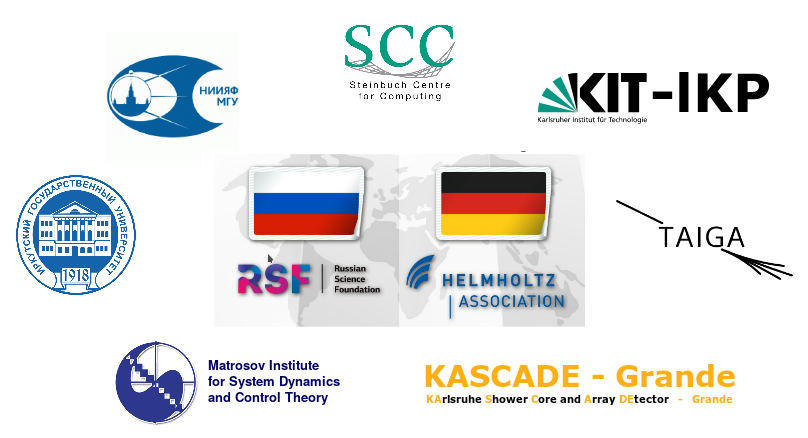
\includegraphics[width=1\linewidth]{pics/Collab.png}
\end{center}
\vspace{-2\parsep}
%     \caption{\small The frist Russian-German big data collaboration}
%     \label{ris:image}
%     \end{figure}
The first Russian-German big data collaboration
\end{frame}

\begin{frame}{KASCASE}
\begin{itemize}
 \item Proposed in 1989 - disassembled in 2013;
 \item Aimed at studying processes at the edge of the Galaxy and beoynd by observing extended atmospheric showers (EAS);
 \item Consisted of:
 \begin{itemize}
  \item scintillators detecting $e$, $\gamma$, $\mu$:
 \begin{itemize}
  %сцинтиляторы, различают e, gamma, mu
    \item KASCADE - 256 stations;
    \item GRANDE - 37 stations;
 \end{itemize}
 %один большой калориметр
    \item Hadronic callorimeter;
 %радиодетектор
    \item Radiodetector LOPES detecting $e$, $e^{+}$;
% позволяющих наблюдать различные компоненты ливня
 \end{itemize}
  \item Significant astrophysical results were obtained. The data analysis is ongoing;
%  благодаря данным с эксперимента было открыто много всего ополезного, при этом анлиз данных продолжается. новые статьи выходят
  \item At the moment all the data collected are available online through the dedicated portal KCDC (KASCADE Cosmic Ray Data Center).
%   к настоящему времени все данные эксперимента опубликованы и доступны онлайн, для этих целей был сделан
%  принциально принципиально новый и крутой на тот момент портал KCDC
% \textcolor{red!50!black}{Add the kcdc logo in the center of the slide}
\end{itemize}

\parbox[t][0pt]{0pt}{
  \vspace{-0.6\textheight}
  ~\hspace{0.68\textwidth}
\includegraphics[width=0.3\textwidth]{pics/KCDC-logo.png}
}
\end{frame}

\begin{frame}{TUNKA}
\footnotesize
\begin{itemize}
 \item Started in the mid 90s and still operating;
 \item Currnlty consists of 4 detectors presented + TUNKA IACT is under construction;
\end{itemize}
\vspace{-1em}
\begin{minipage}[t]{0.48\textwidth}
  \begin{block}{Tunka-133}
    %=============================================
    %=============================================
  \parbox{0.43\textwidth}{
    \centering
    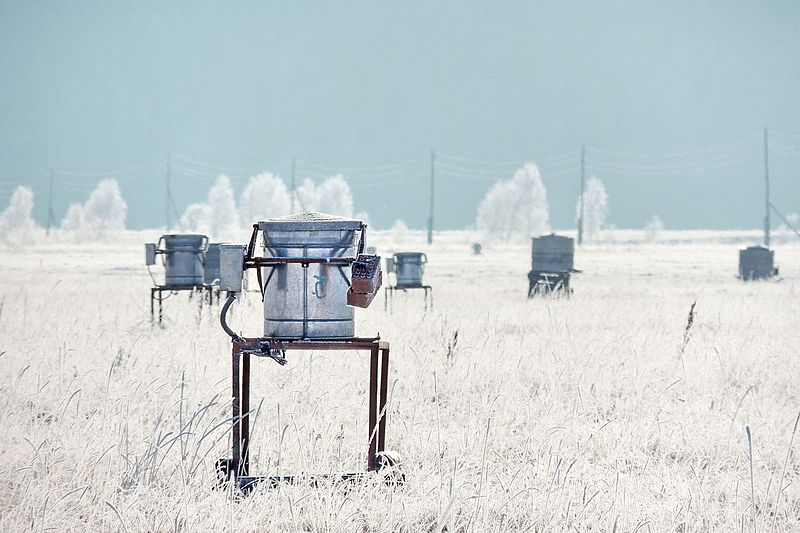
\includegraphics[width=0.48\textwidth]{pics/Tunka-133.jpg}}
% \hfill
\parbox{0.55\textwidth}{
    \begin{itemize}
      \setlength{\itemsep}{0pt}
      \item 133 photomultipliers
      \item measures EAS Cherenkov light
    \end{itemize}
}
    %=============================================
    %=============================================
  \end{block}
\end{minipage}
\hfill
\begin{minipage}[t]{0.48\textwidth}
  \begin{block}{Tunka-Rex}
    %=============================================
    %=============================================
    \parbox{0.43\textwidth}{
        \centering
        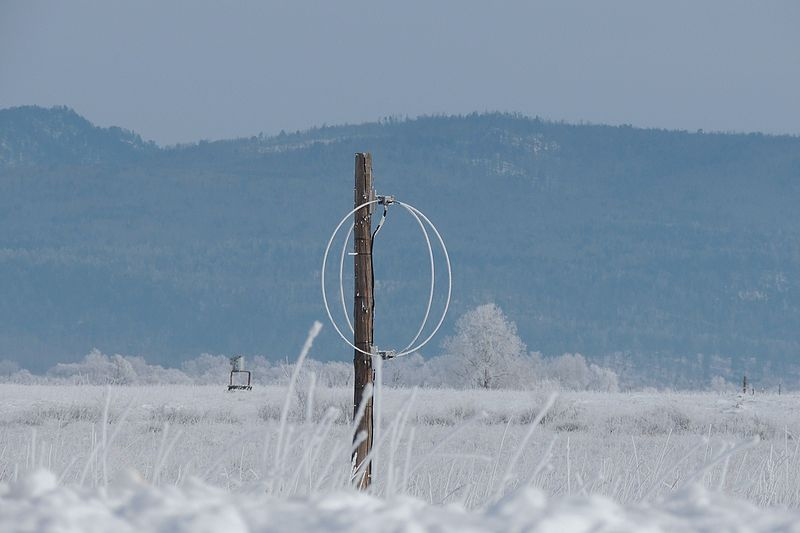
\includegraphics[height=0.22\textheight]{pics/Tunka-Rex.jpg}
    }
    % \hfill
    \parbox{0.55\textwidth}{
        \begin{itemize}
            \setlength{\itemsep}{0pt}
            \item 63 antennas
            \item measures EAS radio-emission
            \vspace{1em}
        \end{itemize}
    }
    %=============================================
    %=============================================
  \end{block}
\end{minipage}

\vspace{-1ex}
\begin{minipage}[t]{0.48\textwidth}
  \begin{block}{Tunka-Grande}
    %=============================================
    %=============================================
    \parbox{0.45\textwidth}{
    \centering
    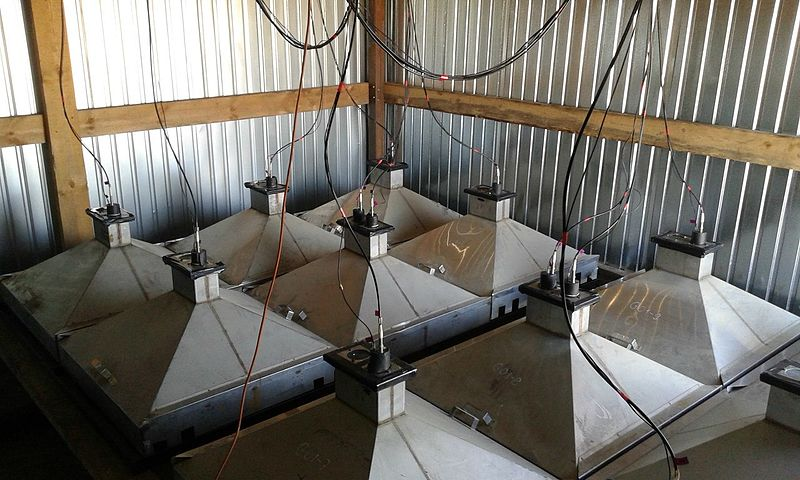
\includegraphics[height=0.23\textheight]{pics/Hiller_Roman-005.jpg}
%     \vspace{-2ex}
        }
    % \hfill
    \parbox{0.5\textwidth}{
    \begin{itemize}
      \setlength{\itemsep}{0pt}
      \item 380 scintillators 0.64m$^2$ each
      \item measures $e$/$\mu$ from EAS
    \end{itemize}
}
    %=============================================
    %=============================================
  \end{block}
\end{minipage}
\hfill
\begin{minipage}[t]{0.48\textwidth}
  \begin{block}{Tunka-HiSCORE}
    %=============================================
    %=============================================
    \parbox{0.43\textwidth}{
    \centering
    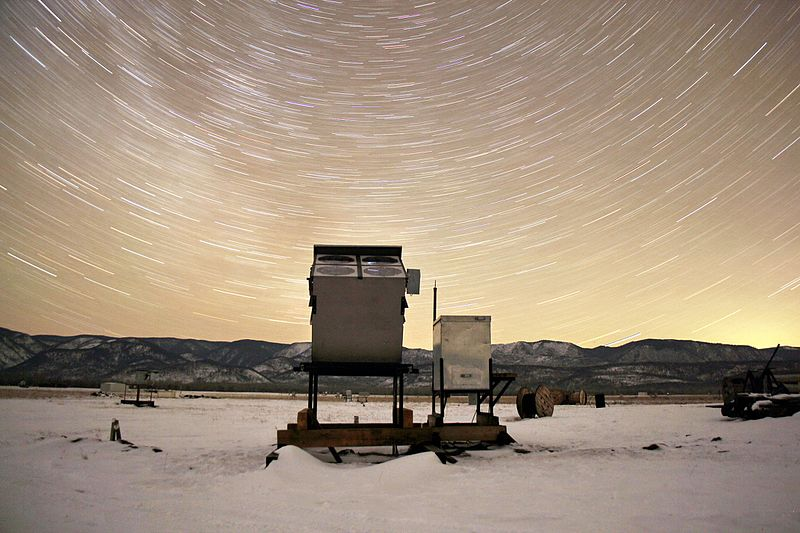
\includegraphics[height=0.23\textheight]{pics/Tunka-HiSCORE.jpg}
%     \vspace{-2ex}
    }
    % \hfill
    \parbox{0.55\textwidth}{
    \begin{itemize}
      \setlength{\itemsep}{0pt}
      \item 47 photomultipliers
      \item measures EAS Cherenkov light
    \end{itemize}
    }
    %=============================================
    %=============================================
  \end{block}
\end{minipage}


\end{frame}

%
% \begin{frame}
%  \begin{exampleblock}{title}
%   text
%  \end{exampleblock}
%
% \end{frame}
